The crossover Core is the next part in the genetics accelerator after the selection cores.
Two inputs are forwarded from the two selections cores as "parents", and two outputs are the "children" of the inputs, containing bits from both parents.
All the bits from both the parents are forwarded in the children, but in some parts the bit-patterns are switched on the children, based a selected crossover function and on a random input from the PRNG.
Henceforth this is called crossover.

There are three distinct crossover functions that are implented: Split, double-split and function.


\paragraph{\textit{Split Fucntion}}
\begin{figure}[H]
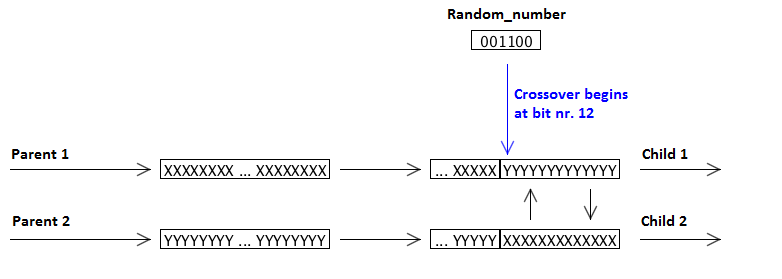
\includegraphics[width=\textwidth]{fpga/fig/crossover_split.png}
\caption{Crossover split function}
\label{fig_crossover_split}
\end{figure}

The first function, crossover split, performs crossover from a selected bit number in the children and until the edge (bit number 0).
This can be seen in figure \ref{fig_crossover_split}.
The values in the parents are represented with X's and Y's, and a single X or Y can have the value 0 or 1, independent of each other.
The bit number for starting crossover is based on the value of a 6-bit input random\_number, which is provided by the PRNG.
This value ranges from 0 to 63.

\begin{figure}[H]
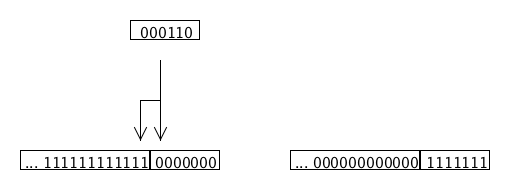
\includegraphics[width=\textwidth]{fpga/fig/crossover_split_mask.png}
\caption{Masking for split function}
\label{fig_crossover_split_mask}
\end{figure}

The split function uses a ShifterVariable, that uses the random\_number for input, and yields an output that consists of 1's until the selected bit number, and 0's on the rest.
Figure \ref{fig_crossover_split_mask} shows an example where bit nr.
6 is selected for beginning crossover, and bits 6-0 in the output consist of 0's, and the rest 1's.
This output is called \emph{mask1}.
\emph{Mask2} is set as a negated \emph{mask1}, so the bits in \emph{mask2} would be 1's where they would be 0's in the other, and vice versa.
Only bits 6-0 would be 1's in \emph{mask2} in the figure.
The output on the children are set by combininging the parents and the masks:
\linebreak child1 \<= (parent1 and mask1) or (parent2 and mask2);
\linebreak child2 \<= (parent1 and mask2) or (parent2 and mask1);
\todo{ Would be more simple to show the code line, though maybe not as elegant as writing an elaborative text, but is there any other better reason to explain this by text?}

\todo{ "Selected bit number" needs to somehow be defined in the description of the shifter variable + ShifterVariable needs to be described.}

\paragraph{\textit{Double-split Fucntion}}
\begin{figure}[H]
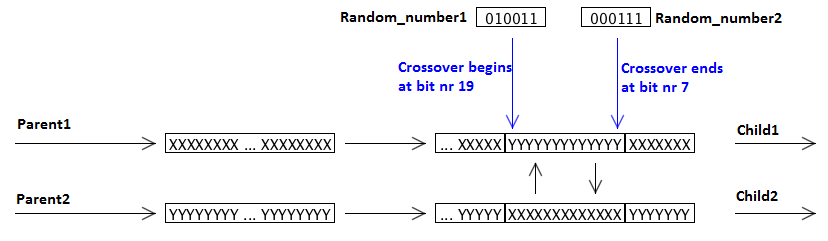
\includegraphics[width=\textwidth]{fpga/fig/crossover_doublesplit.png}
\caption{Crossover double-split function}
\label{fig_crossover_doublesplit}
\end{figure}

The second function, crossover double-split, is similar to the crossover\_split-function, but in additionally to having a starting bit for crossover, it also has an ending bit where the crossover starts, instead of reaching the edge at bit nr.
0.
PRNG provides with 2 6-bit inputs, random\_number1 and random\_number2, whose values selects the starting bit and the ending bit for the crossover.
These values range from 0 to 63, and if both are the same, then only one bit will be selected for crossover.

\begin{figure}[H]
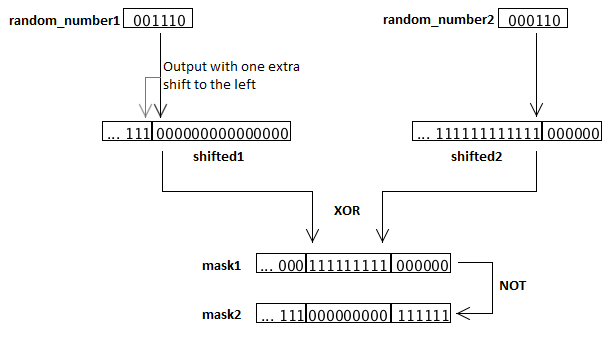
\includegraphics[width=\textwidth]{fpga/fig/crossover_doublesplit_mask.png}
\caption{Masking for double-split function}
\label{fig_crossover_doublesplit_mask}
\end{figure}

The double-split function uses two ShifterVariables, which take an input each from the random\_numbers.
The ShifterVariables are used in the same ways as in the split function, but the outputs will differ from each other as to where the transition from 1's to 0's are set.
One will have more 1's than the other (at least one if both the random numbers are the same).
The masks are set by using XOR-function of the outputs, so that \emph{mask1} will have 0's with both the MS and the LS portions of bits, but with a area of 1's between, and \emph{mask2} is it's negation.
Figure \ref{fig_crossover_doublesplit_mask} provides such an example, where bits number 14 and 6 are selected.
The bits 14-6 in \emph{mask1} would be 1's and the rest 0's by using XOR-function with the outputs from the ShifterVariables, and vice versa in \emph{mask2} by setting it as the negation of \emph{mask1}.
The final outputs are set the same way as in the split function.

\todo{ Ugh....still klutzy}
\todo{ ShifterVariable needs to be described.}

\paragraph{\textit{XOR Fucntion}}
\begin{figure}[H]
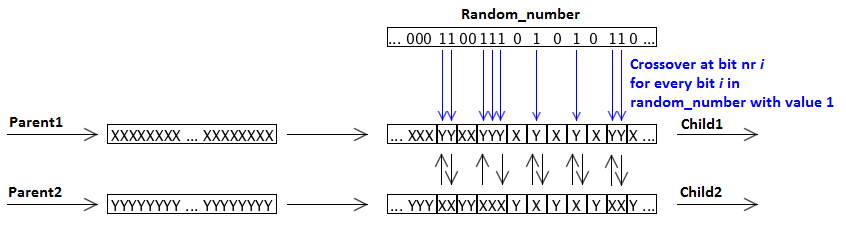
\includegraphics[width=\textwidth]{fpga/fig/crossover_xor.png}
\caption{Crossover XOR function}
\label{fig_crossover_xor}
\end{figure}

The third function, crossover XOR, performs crossover bit by bit, based on the 64-bit input random\_number.
For each bit number \emph{i} in random\_number that has the value 1, the function will perform crossover on the children at the same bit number \emph{i}.
This function is called XOR because of use of XOR-gates in earlier version of the function, and the principle is still the same: For each bit number \emph{i} in the child, the value will the bit number \emph{i} from one and only one parent.
And which parent it is depends on the value of bit number \emph{i} in random\_number.

\paragraph{\textit{Crossover Core Toplevel}}

The crossover core is implemented on the genetics accelerator as a toplevel containing 3 subcores, one for each function, as well as a fourth path with no crossover.
In addition to the two parent inputs and 64-bit input random\_number, the toplevel has a control\_number input used for determining which crossover function is to be used: Split, doublesplit, xor, "party mode" or no crossover at all.
Party mode is choosing crossover function at random, based on the 2 LS bits in the random\_number.
In this way, whenever inputs are sent through the crossover\_toplevel, different functions may be used at different times.
These are the control values:
\begin{itemize}
\item 000 - Split
\item 001 - Double-split
\item 010 - XOR
\item 011 - No crossover
\item 1XX - Party mode, in which case these are the random control values:
    \begin{itemize}
    \item 00 - Split
    \item 01 - Doublesplit
    \item 10 - XOR
    \item 11 - No crossover
    \end{itemize}
\end{itemize}
